\documentclass[12pt,]{article}
\usepackage{lmodern}
\usepackage{amssymb,amsmath}
\usepackage{ifxetex,ifluatex}
\usepackage{fixltx2e} % provides \textsubscript
\ifnum 0\ifxetex 1\fi\ifluatex 1\fi=0 % if pdftex
  \usepackage[T1]{fontenc}
  \usepackage[utf8]{inputenc}
\else % if luatex or xelatex
  \ifxetex
    \usepackage{mathspec}
  \else
    \usepackage{fontspec}
  \fi
  \defaultfontfeatures{Ligatures=TeX,Scale=MatchLowercase}
    \setmainfont[]{Times New Roman}
\fi
% use upquote if available, for straight quotes in verbatim environments
\IfFileExists{upquote.sty}{\usepackage{upquote}}{}
% use microtype if available
\IfFileExists{microtype.sty}{%
\usepackage{microtype}
\UseMicrotypeSet[protrusion]{basicmath} % disable protrusion for tt fonts
}{}
\usepackage[margin=2.54cm]{geometry}
\usepackage{hyperref}
\hypersetup{unicode=true,
            pdftitle={Changes in Land Use between 1990 and 2014},
            pdfauthor={Rebecca Marx},
            pdfborder={0 0 0},
            breaklinks=true}
\urlstyle{same}  % don't use monospace font for urls
\usepackage{color}
\usepackage{fancyvrb}
\newcommand{\VerbBar}{|}
\newcommand{\VERB}{\Verb[commandchars=\\\{\}]}
\DefineVerbatimEnvironment{Highlighting}{Verbatim}{commandchars=\\\{\}}
% Add ',fontsize=\small' for more characters per line
\usepackage{framed}
\definecolor{shadecolor}{RGB}{248,248,248}
\newenvironment{Shaded}{\begin{snugshade}}{\end{snugshade}}
\newcommand{\KeywordTok}[1]{\textcolor[rgb]{0.13,0.29,0.53}{\textbf{#1}}}
\newcommand{\DataTypeTok}[1]{\textcolor[rgb]{0.13,0.29,0.53}{#1}}
\newcommand{\DecValTok}[1]{\textcolor[rgb]{0.00,0.00,0.81}{#1}}
\newcommand{\BaseNTok}[1]{\textcolor[rgb]{0.00,0.00,0.81}{#1}}
\newcommand{\FloatTok}[1]{\textcolor[rgb]{0.00,0.00,0.81}{#1}}
\newcommand{\ConstantTok}[1]{\textcolor[rgb]{0.00,0.00,0.00}{#1}}
\newcommand{\CharTok}[1]{\textcolor[rgb]{0.31,0.60,0.02}{#1}}
\newcommand{\SpecialCharTok}[1]{\textcolor[rgb]{0.00,0.00,0.00}{#1}}
\newcommand{\StringTok}[1]{\textcolor[rgb]{0.31,0.60,0.02}{#1}}
\newcommand{\VerbatimStringTok}[1]{\textcolor[rgb]{0.31,0.60,0.02}{#1}}
\newcommand{\SpecialStringTok}[1]{\textcolor[rgb]{0.31,0.60,0.02}{#1}}
\newcommand{\ImportTok}[1]{#1}
\newcommand{\CommentTok}[1]{\textcolor[rgb]{0.56,0.35,0.01}{\textit{#1}}}
\newcommand{\DocumentationTok}[1]{\textcolor[rgb]{0.56,0.35,0.01}{\textbf{\textit{#1}}}}
\newcommand{\AnnotationTok}[1]{\textcolor[rgb]{0.56,0.35,0.01}{\textbf{\textit{#1}}}}
\newcommand{\CommentVarTok}[1]{\textcolor[rgb]{0.56,0.35,0.01}{\textbf{\textit{#1}}}}
\newcommand{\OtherTok}[1]{\textcolor[rgb]{0.56,0.35,0.01}{#1}}
\newcommand{\FunctionTok}[1]{\textcolor[rgb]{0.00,0.00,0.00}{#1}}
\newcommand{\VariableTok}[1]{\textcolor[rgb]{0.00,0.00,0.00}{#1}}
\newcommand{\ControlFlowTok}[1]{\textcolor[rgb]{0.13,0.29,0.53}{\textbf{#1}}}
\newcommand{\OperatorTok}[1]{\textcolor[rgb]{0.81,0.36,0.00}{\textbf{#1}}}
\newcommand{\BuiltInTok}[1]{#1}
\newcommand{\ExtensionTok}[1]{#1}
\newcommand{\PreprocessorTok}[1]{\textcolor[rgb]{0.56,0.35,0.01}{\textit{#1}}}
\newcommand{\AttributeTok}[1]{\textcolor[rgb]{0.77,0.63,0.00}{#1}}
\newcommand{\RegionMarkerTok}[1]{#1}
\newcommand{\InformationTok}[1]{\textcolor[rgb]{0.56,0.35,0.01}{\textbf{\textit{#1}}}}
\newcommand{\WarningTok}[1]{\textcolor[rgb]{0.56,0.35,0.01}{\textbf{\textit{#1}}}}
\newcommand{\AlertTok}[1]{\textcolor[rgb]{0.94,0.16,0.16}{#1}}
\newcommand{\ErrorTok}[1]{\textcolor[rgb]{0.64,0.00,0.00}{\textbf{#1}}}
\newcommand{\NormalTok}[1]{#1}
\usepackage{longtable,booktabs}
\usepackage{graphicx,grffile}
\makeatletter
\def\maxwidth{\ifdim\Gin@nat@width>\linewidth\linewidth\else\Gin@nat@width\fi}
\def\maxheight{\ifdim\Gin@nat@height>\textheight\textheight\else\Gin@nat@height\fi}
\makeatother
% Scale images if necessary, so that they will not overflow the page
% margins by default, and it is still possible to overwrite the defaults
% using explicit options in \includegraphics[width, height, ...]{}
\setkeys{Gin}{width=\maxwidth,height=\maxheight,keepaspectratio}
\IfFileExists{parskip.sty}{%
\usepackage{parskip}
}{% else
\setlength{\parindent}{0pt}
\setlength{\parskip}{6pt plus 2pt minus 1pt}
}
\setlength{\emergencystretch}{3em}  % prevent overfull lines
\providecommand{\tightlist}{%
  \setlength{\itemsep}{0pt}\setlength{\parskip}{0pt}}
\setcounter{secnumdepth}{5}
% Redefines (sub)paragraphs to behave more like sections
\ifx\paragraph\undefined\else
\let\oldparagraph\paragraph
\renewcommand{\paragraph}[1]{\oldparagraph{#1}\mbox{}}
\fi
\ifx\subparagraph\undefined\else
\let\oldsubparagraph\subparagraph
\renewcommand{\subparagraph}[1]{\oldsubparagraph{#1}\mbox{}}
\fi

%%% Use protect on footnotes to avoid problems with footnotes in titles
\let\rmarkdownfootnote\footnote%
\def\footnote{\protect\rmarkdownfootnote}

%%% Change title format to be more compact
\usepackage{titling}

% Create subtitle command for use in maketitle
\providecommand{\subtitle}[1]{
  \posttitle{
    \begin{center}\large#1\end{center}
    }
}

\setlength{\droptitle}{-2em}

  \title{Changes in Land Use between 1990 and 2014}
    \pretitle{\vspace{\droptitle}\centering\huge}
  \posttitle{\par}
  \subtitle{\url{https://github.com/RsMarx/Ag_Forest_Data_Final-}}
  \author{Rebecca Marx}
    \preauthor{\centering\large\emph}
  \postauthor{\par}
    \date{}
    \predate{}\postdate{}
  

\begin{document}
\maketitle
\begin{abstract}
Experimental overview. This section should be no longer than 250 words.
\end{abstract}

\newpage

\tableofcontents  \newpage
\listoftables  \newpage
\listoffigures  \newpage

\textless{}Note: set up autoreferencing for figures and tables in your
document\textgreater{}

\section{Research Question and
Rationale}\label{research-question-and-rationale}

As the global population continues to grow and require more food and
fuel resources, deforestation trends are expected to accelerate.
Deforestation can be problematic as forests provide ecosystem services
such as carbon storage, nutrient cycling, water filtration, and wildlife
habitat. Agriculture is one of the most commonly sited drivers of
deforestation, in addition to being a source of emissions. Given that
forest and agriculture can be contending land uses, this research
examines the relationship between agriculture and forest as land uses
and, more broadly, explores the causes and impacts of changes in land
use.

This research looks at the trends and tradeoffs in land use across
countries from 1990 -- 2014. Primary questions include:

\begin{itemize}
\tightlist
\item
  Is there a relationship between the percentage of land area dedicated
  to forest versus agricultural in countries?
\item
  Is there a relationship between land uses (agriculture or forest) and
  levels of CO2, methane, and NO3 emissions?
\item
  Is there a relationship between access to electricity or renewable
  electricity output and the percentage of land dedicated to forestry
  versus agriculture?
\end{itemize}

The research utilizes a data set from the World Bank that has 135
environment-related variables for 264 countries. I have narrowed the
environment variable down to 7 that are relevant to land use. Although
the full data set dates back to 1960, I have limited to the time scope
of the analysis to between 1990 and 2014 because those are the dates for
which forest cover data is available.

\newpage

\section{Dataset Information}\label{dataset-information}

\subsection{Database Information}\label{database-information}

Data were collected from the World Bank website. More information can be
found here: \url{https://data.worldbank.org/topic/environment} Data were
downloaded as a full data set called
``API\_6\_DS2\_en\_csv\_v2\_10518155''. The csv file was saved as
``WorldBank\_Raw\_4.8.19''. Variables from among the raw data set were
selected to be used in the data set analysed. Only 7 of a possible 135
environment-related variables were retained in the processed data. This
csv file was saved as {[}``WorldBank\_Processed''; ``WorldBank\_Spread''
or ``WB\_Spread''{]}.

\subsection{Data Content Information}\label{data-content-information}

Country: Originally named ``Country.Name'', the Country variable
includes 264 countries.

Year: The Year variable was originally spread horizontally from 1960 --
2018. The years were gathered in to one column named ``Year'' and
formatted as a date.

Forest: The Forest variable was originally named ``Forest area (\% of
land area)''. Its data range is 1990 -- 2016.

Agriculture: The Agriculture variable was originally named ``Agriculture
land (\% of land area). Its data range is from 1961 -- 2018.

Ag.Methane: The Ag.Methane variable was originally named ``Agriculture
methane emissions (thousand metric tons of CO2 equivalent). Its data
range is 1970 -- 2008.

Ag.NO2: The Ag.NO2 variable was originally named ``Agriculture nitrous
oxide emissions (thousand metric tons of CO2 equivalent). Its data range
is 1970 -- 2008.

CO2Emissions: The CO2Emissions variable was originally named ``CO2
emissions (kt). Its data range is 1960 -- 2014.

ElectricityAccess: The ElectricityAccess variable was originally named
``Access to electricity (\% of total population). Data range is 1990 --
2016.

RenewableElectricity: The RenewableElectricity variable was originally
named ``Renewable electricity output (\% of total electricity output).
Its data range is 1990 -- 2015.

\subsection{Naming conventions and file
formats}\label{naming-conventions-and-file-formats}

The files are named according to the following convention:
\texttt{databasename\_datatype\_details\_stage.format}, where: Files are
named according to the following naming convention:
\textbf{databasename} refers to the database from where the data
originated \textbf{details} are additional descriptive details related
to the stage of data wrangling \textbf{stage}refers to the stage in data
management pipelines (e.g., raw or processed) \textbf{format} is a
non-proprietary file format (e.g., .csv, .txt)

\subsection{Additional Information and
Support}\label{additional-information-and-support}

For more information, please contact the data assembler, \textbf{Rebecca
Marx}
(\href{mailto:rebecca.marx@duke.edu}{\nolinkurl{rebecca.marx@duke.edu}})

\begin{longtable}[]{@{}lll@{}}
\toprule
Variable & Units & Data Strcuture\tabularnewline
\midrule
\endhead
Cell 1 & Cell 2 & Cells\tabularnewline
Cell 3 & Cell 4 & Cells\tabularnewline
\bottomrule
\end{longtable}

\newpage

\section{Exploratory Data Analysis and
Wrangling}\label{exploratory-data-analysis-and-wrangling}

Wrangling the data required multiple operations. First, I used the
filter function to select only 9 of a possible 135 variables in the data
set. Since the data set was arranged with the years going horizontally,
I then had to gather the years in to one column, and create a new column
called ``Level'' that contained the values recorded for each variable in
each year.

\begin{Shaded}
\begin{Highlighting}[]
\NormalTok{World_Bank_Master <-}\KeywordTok{read.csv}\NormalTok{(}\StringTok{"../Raw/WorldBank_Raw2_4.8.19.csv"}\NormalTok{)}

\CommentTok{#Data Subset}
\NormalTok{World_Bank_Filter <-}\StringTok{ }\KeywordTok{filter}\NormalTok{(World_Bank_Master, Indicator.Name }\OperatorTok{==}\StringTok{ "Forest area (% of land area)"} \OperatorTok{|}\StringTok{ }\NormalTok{Indicator.Name }\OperatorTok{==}\StringTok{ "Agricultural land (% of land area)"} \OperatorTok{|}\StringTok{ }\NormalTok{Indicator.Name }\OperatorTok{==}\StringTok{ "Access to electricity (% of population)"} \OperatorTok{|}\StringTok{ }\NormalTok{Indicator.Name }\OperatorTok{==}\StringTok{ "Renewable electricity output (% of total electricity output)"} \OperatorTok{|}\StringTok{ }\NormalTok{Indicator.Name }\OperatorTok{==}\StringTok{ "CO2 emissions (kt)"} \OperatorTok{|}\StringTok{ }\NormalTok{Indicator.Name }\OperatorTok{==}\StringTok{ "Agricultural nitrous oxide emissions (thousand metric tons of CO2 equivalent)"} \OperatorTok{|}\StringTok{ }\NormalTok{Indicator.Name }\OperatorTok{==}\StringTok{ "Agricultural methane emissions (thousand metric tons of CO2 equivalent)"}\NormalTok{)}

\NormalTok{WorldBank_Gather <-}\StringTok{ }\KeywordTok{gather}\NormalTok{(World_Bank_Filter, }\StringTok{"Year"}\NormalTok{, }\StringTok{"Level"}\NormalTok{, X1960}\OperatorTok{:}\NormalTok{X2018)}

\NormalTok{WorldBank_Gather <-}\StringTok{ }\KeywordTok{select}\NormalTok{(WorldBank_Gather, }\OperatorTok{-}\NormalTok{Indicator.Code)}

\NormalTok{WorldBank_Spread <-}\StringTok{  }\KeywordTok{spread}\NormalTok{(WorldBank_Gather, Indicator.Name, Level)}

\CommentTok{#Format as character }
\NormalTok{WorldBank_Spread}\OperatorTok{$}\NormalTok{Year <-}\StringTok{ }\KeywordTok{as.character}\NormalTok{(WorldBank_Spread}\OperatorTok{$}\NormalTok{Year)}

\CommentTok{#create string}
\NormalTok{WB_String <-}\StringTok{ }\KeywordTok{substr}\NormalTok{(WorldBank_Spread}\OperatorTok{$}\NormalTok{Year, }\DecValTok{2}\NormalTok{, }\DecValTok{5}\NormalTok{)}

\CommentTok{#Get rid of X in date}
\NormalTok{WorldBank_Spread}\OperatorTok{$}\NormalTok{Year =}\StringTok{ }\NormalTok{WB_String}

\CommentTok{#Format as date}
\CommentTok{#WB_Fixed$Year <- as.Date(WB_Fixed$Year)}
\NormalTok{WorldBank_Spread}\OperatorTok{$}\NormalTok{Year <-}\StringTok{ }\KeywordTok{as.Date}\NormalTok{(WorldBank_Spread}\OperatorTok{$}\NormalTok{Year, }\DataTypeTok{format =} \StringTok{"%Y"}\NormalTok{) }\CommentTok{#can I get it to show only the year? }

\CommentTok{#Change column names }
\KeywordTok{names}\NormalTok{(WorldBank_Spread) <-}\StringTok{ }\KeywordTok{c}\NormalTok{(}\StringTok{"Country"}\NormalTok{, }\StringTok{"Indicator.Code"}\NormalTok{, }\StringTok{"Year"}\NormalTok{, }\StringTok{"ElectricityAccess"}\NormalTok{, }\StringTok{"Agriculture"}\NormalTok{, }\StringTok{"Ag.Methane"}\NormalTok{, }\StringTok{"Ag.NO2"}\NormalTok{, }\StringTok{"CO2Emissions"}\NormalTok{, }\StringTok{"Forest"}\NormalTok{, }\StringTok{"RenewableElectricity"}\NormalTok{)}

\CommentTok{#Save processed file }
\CommentTok{#write.csv(WorldBank_Spread, row.names = FALSE, file = "../Processed/WorldBank_Processed.csv")}
   
\NormalTok{Five_Countries <-}\StringTok{ }\KeywordTok{filter}\NormalTok{(WorldBank_Spread, Country }\OperatorTok{==}\StringTok{ "Brazil"} \OperatorTok{|}\StringTok{ }\NormalTok{Country }\OperatorTok{==}\StringTok{ "Kenya"} \OperatorTok{|}\StringTok{ }\NormalTok{Country }\OperatorTok{==}\StringTok{ "Spain"} \OperatorTok{|}\StringTok{ }\NormalTok{Country }\OperatorTok{==}\StringTok{ "Indonesia"} \OperatorTok{|}\StringTok{ }\NormalTok{Country }\OperatorTok{==}\StringTok{ "Canada"}\NormalTok{)}

\NormalTok{WB_Spread <-}\StringTok{ }\NormalTok{WorldBank_Spread }\OperatorTok\StringTok{ }
\StringTok{  }\NormalTok{na.exclude }\CommentTok{#check if I need this for my tests}

\NormalTok{WB_Brazil <-}\StringTok{ }\KeywordTok{filter}\NormalTok{(WB_Spread, Country }\OperatorTok{==}\StringTok{ "Brazil"}\NormalTok{)}
\end{Highlighting}
\end{Shaded}

\begin{verbatim}

<Include R chunks for 5+ lines of summary code (display code and output), 3+ exploratory graphs (display graphs only), and any wrangling you do to your dataset(s).> 

\end{verbatim}

After the data was wrangled into a format that would function well with
my intended R operations, I was able to begin exploring the data set.

\begin{Shaded}
\begin{Highlighting}[]
\CommentTok{#5+ lines of summary }

\KeywordTok{colnames}\NormalTok{(WorldBank_Spread)}
\end{Highlighting}
\end{Shaded}

\begin{verbatim}
##  [1] "Country"              "Indicator.Code"       "Year"                
##  [4] "ElectricityAccess"    "Agriculture"          "Ag.Methane"          
##  [7] "Ag.NO2"               "CO2Emissions"         "Forest"              
## [10] "RenewableElectricity"
\end{verbatim}

\begin{Shaded}
\begin{Highlighting}[]
\KeywordTok{class}\NormalTok{(WorldBank_Spread}\OperatorTok{$}\NormalTok{Year)}
\end{Highlighting}
\end{Shaded}

\begin{verbatim}
## [1] "Date"
\end{verbatim}

\begin{Shaded}
\begin{Highlighting}[]
\KeywordTok{dim}\NormalTok{(WorldBank_Spread)}
\end{Highlighting}
\end{Shaded}

\begin{verbatim}
## [1] 15576    10
\end{verbatim}

\begin{Shaded}
\begin{Highlighting}[]
\KeywordTok{head}\NormalTok{(WorldBank_Spread)}
\end{Highlighting}
\end{Shaded}

\begin{verbatim}
##       Country Indicator.Code       Year ElectricityAccess Agriculture
## 1 Afghanistan            AFG 1960-04-15                NA          NA
## 2 Afghanistan            AFG 1961-04-15                NA    57.74592
## 3 Afghanistan            AFG 1962-04-15                NA    57.83782
## 4 Afghanistan            AFG 1963-04-15                NA    57.91441
## 5 Afghanistan            AFG 1964-04-15                NA    58.01091
## 6 Afghanistan            AFG 1965-04-15                NA    58.01397
##   Ag.Methane Ag.NO2 CO2Emissions Forest RenewableElectricity
## 1         NA     NA      414.371     NA                   NA
## 2         NA     NA      491.378     NA                   NA
## 3         NA     NA      689.396     NA                   NA
## 4         NA     NA      707.731     NA                   NA
## 5         NA     NA      839.743     NA                   NA
## 6         NA     NA     1008.425     NA                   NA
\end{verbatim}

\begin{Shaded}
\begin{Highlighting}[]
\KeywordTok{summary}\NormalTok{(WorldBank_Spread)}
\end{Highlighting}
\end{Shaded}

\begin{verbatim}
##            Country      Indicator.Code       Year           
##  Afghanistan   :   59   ABW    :   59   Min.   :1960-04-15  
##  Albania       :   59   AFG    :   59   1st Qu.:1974-04-15  
##  Algeria       :   59   AGO    :   59   Median :1989-04-15  
##  American Samoa:   59   ALB    :   59   Mean   :1989-04-14  
##  Andorra       :   59   AND    :   59   3rd Qu.:2004-04-15  
##  Angola        :   59   ARB    :   59   Max.   :2018-04-15  
##  (Other)       :15222   (Other):15222                       
##  ElectricityAccess  Agriculture        Ag.Methane          Ag.NO2         
##  Min.   :  0.00    Min.   : 0.2628   Min.   :      0   Min.   :      0.0  
##  1st Qu.: 53.11    1st Qu.:20.5547   1st Qu.:    120   1st Qu.:     86.9  
##  Median : 93.94    Median :37.3659   Median :   3300   Median :   2302.9  
##  Mean   : 75.04    Mean   :37.0790   Mean   : 117609   Mean   :  63590.8  
##  3rd Qu.:100.00    3rd Qu.:52.3930   3rd Qu.:  24198   3rd Qu.:  15076.6  
##  Max.   :100.00    Max.   :93.4407   Max.   :3464398   Max.   :2242932.7  
##  NA's   :8618      NA's   :2521      NA's   :5056      NA's   :5056       
##   CO2Emissions          Forest         RenewableElectricity
##  Min.   :     -81   Min.   :    0.00   Min.   :  0.000     
##  1st Qu.:     964   1st Qu.:   12.50   1st Qu.:  0.465     
##  Median :   11463   Median :   31.18   Median : 16.961     
##  Mean   :  736069   Mean   :   42.70   Mean   : 28.211     
##  3rd Qu.:  143107   3rd Qu.:   46.96   3rd Qu.: 49.255     
##  Max.   :36138285   Max.   :16735.00   Max.   :100.000     
##  NA's   :3321       NA's   :8717       NA's   :8738
\end{verbatim}

\begin{Shaded}
\begin{Highlighting}[]
\KeywordTok{summary}\NormalTok{(WorldBank_Spread}\OperatorTok{$}\NormalTok{Agriculture)}
\end{Highlighting}
\end{Shaded}

\begin{verbatim}
##    Min. 1st Qu.  Median    Mean 3rd Qu.    Max.    NA's 
##  0.2628 20.5547 37.3659 37.0790 52.3930 93.4407    2521
\end{verbatim}

\begin{Shaded}
\begin{Highlighting}[]
\KeywordTok{summary}\NormalTok{(WorldBank_Spread}\OperatorTok{$}\NormalTok{Forest)}
\end{Highlighting}
\end{Shaded}

\begin{verbatim}
##     Min.  1st Qu.   Median     Mean  3rd Qu.     Max.     NA's 
##     0.00    12.50    31.18    42.70    46.96 16735.00     8717
\end{verbatim}

\begin{Shaded}
\begin{Highlighting}[]
\KeywordTok{summary}\NormalTok{(WorldBank_Spread}\OperatorTok{$}\NormalTok{RenewableElectricty)}
\end{Highlighting}
\end{Shaded}

\begin{verbatim}
## Length  Class   Mode 
##      0   NULL   NULL
\end{verbatim}

\begin{Shaded}
\begin{Highlighting}[]
\KeywordTok{summary}\NormalTok{(WB_Spread}\OperatorTok{$}\NormalTok{Ag.Methane)}
\end{Highlighting}
\end{Shaded}

\begin{verbatim}
##    Min. 1st Qu.  Median    Mean 3rd Qu.    Max. 
##       0     687    4638  138432   36696 3464398
\end{verbatim}

(Figure\ref{fig:fig1}) plots agriculture and forest land covers to see
if there is a noticable trend. It appears that there is a tendency for
forest cover to decrease as agriculture cover increases.

\begin{verbatim}
## function (expr) 
## {
##     enexpr(expr)
## }
## <bytecode: 0x000000001a9610c8>
## <environment: namespace:rlang>
\end{verbatim}

\begin{verbatim}
## Warning: Removed 8897 rows containing missing values (geom_point).
\end{verbatim}

\begin{figure}
\centering
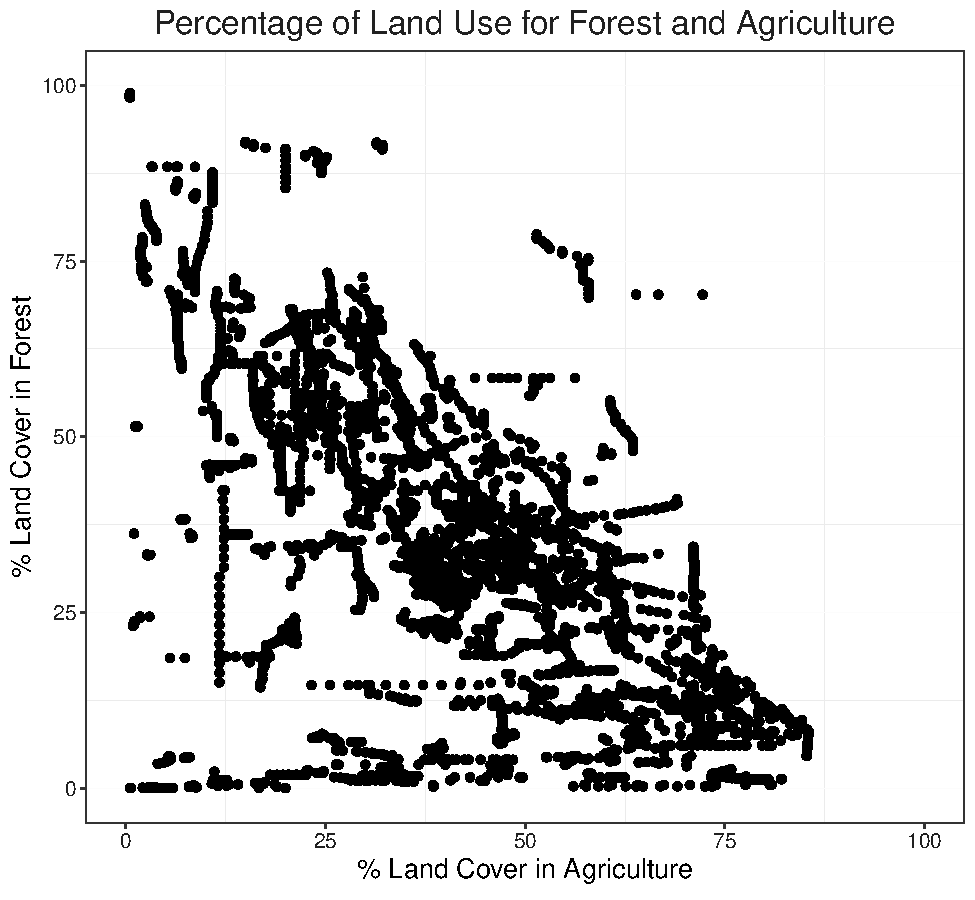
\includegraphics{Marx_ENV872_Project_files/figure-latex/fig1-1.pdf}
\caption{\label{fig:fig1}Percentage of Land Use for Forest and
Agriculture}
\end{figure}

A second exploratory graph plots forest levels for all 264 countries
over time. The resulting graph shows that there is some movement over
time, but many countries see constant levels of land use. In later
graphs I decided to reduce the number of countries included to be able
to better visualized changes. Similarly, a plot of agriculture over time
shows some movement over time, but many countries see constant levels of
land use for agriculture.

\begin{verbatim}
## function (expr) 
## {
##     enexpr(expr)
## }
## <bytecode: 0x000000001a9610c8>
## <environment: namespace:rlang>
\end{verbatim}

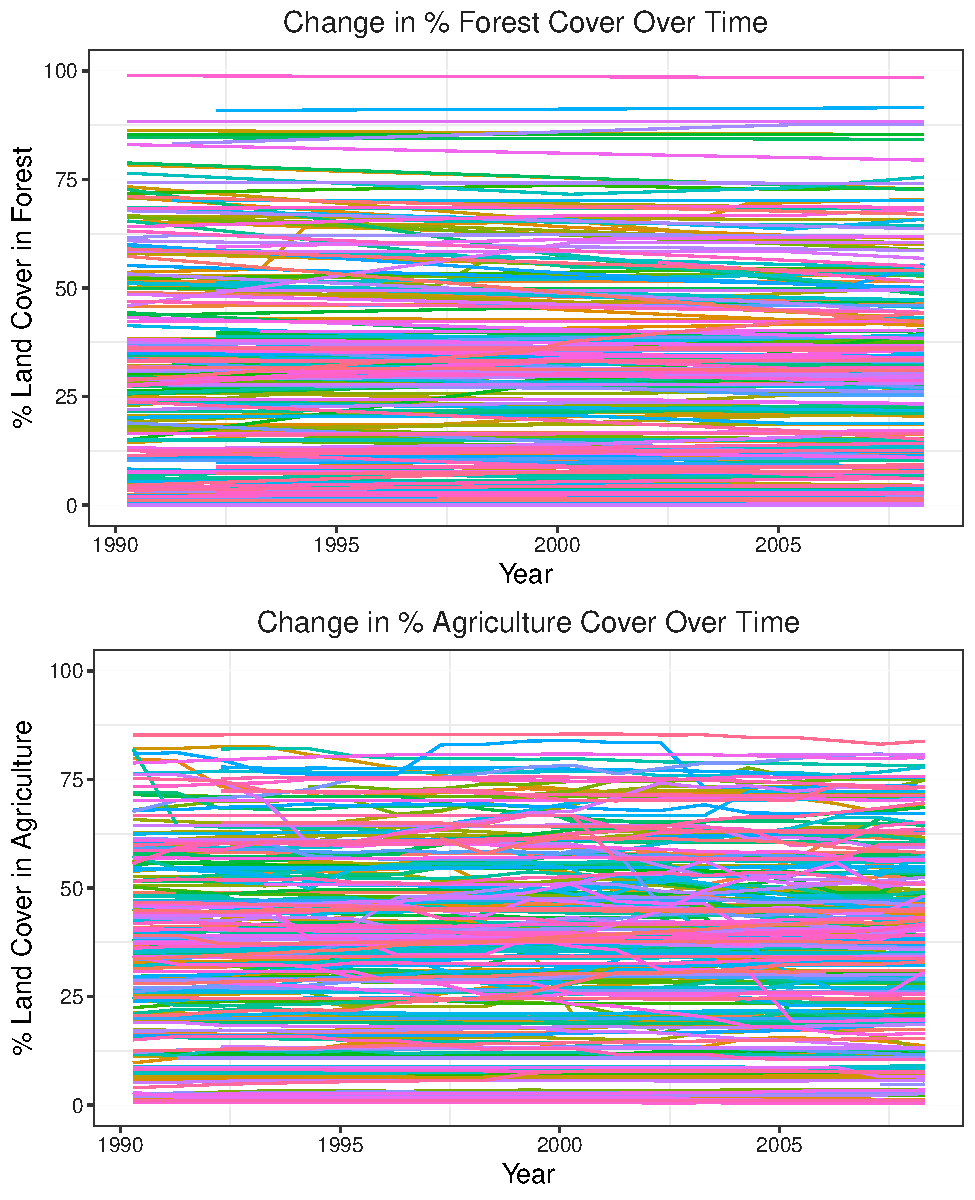
\includegraphics{Marx_ENV872_Project_files/figure-latex/unnamed-chunk-3-1.pdf}
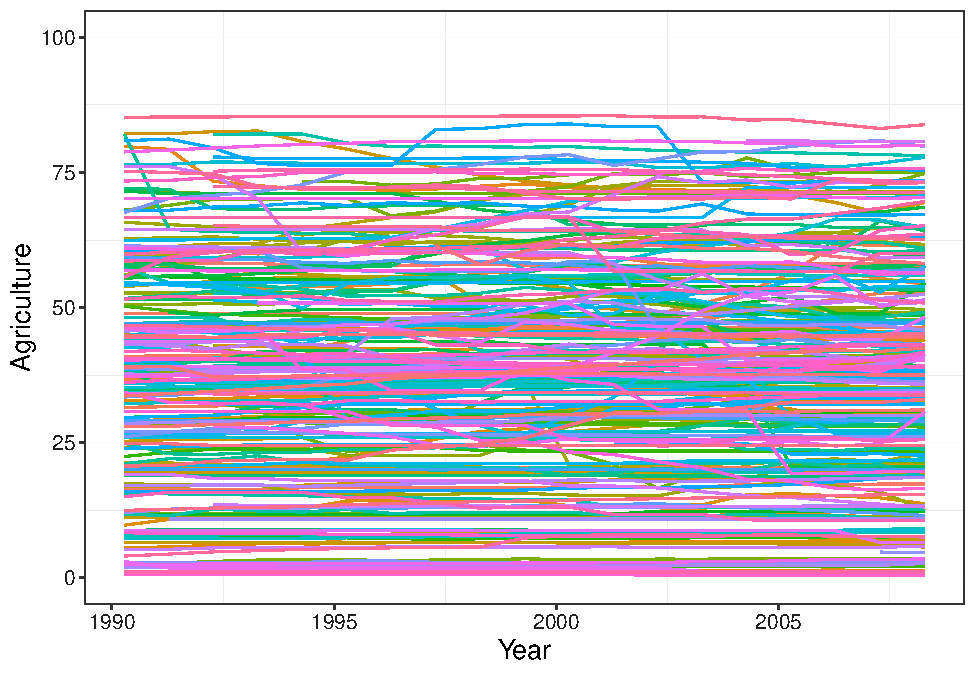
\includegraphics{Marx_ENV872_Project_files/figure-latex/unnamed-chunk-3-2.pdf}
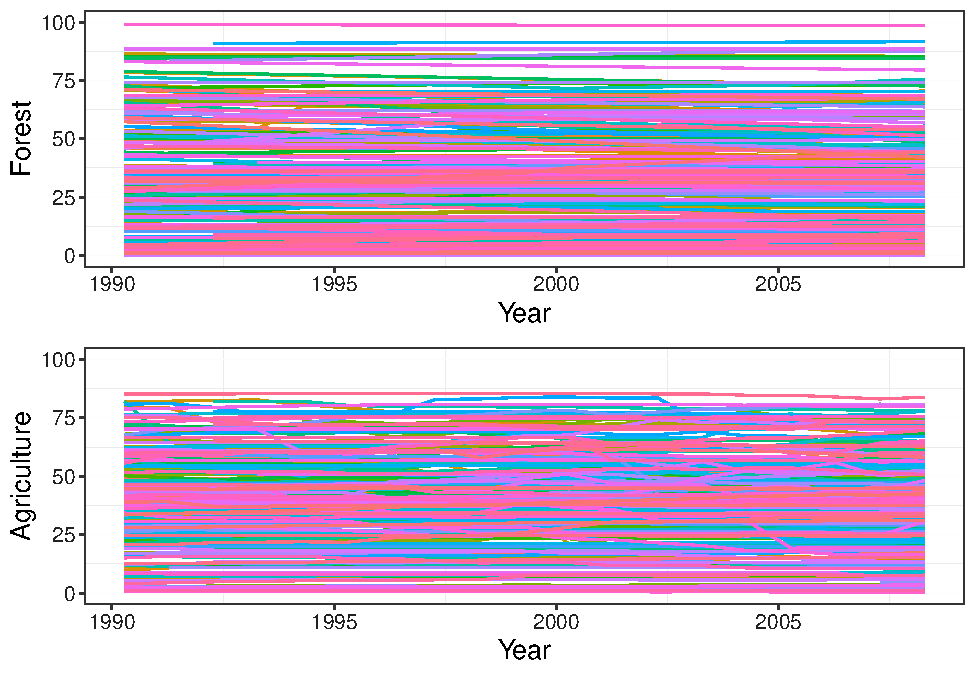
\includegraphics{Marx_ENV872_Project_files/figure-latex/unnamed-chunk-3-3.pdf}

Since the research attempts to decipher whether a change in forest
levels is related to a change in agriculture levels, I also wanted to
see if a change in the amount of land dedicated to agriculture leads to
a change in various emissions levels. The following graphs explore these
relationships.

\begin{verbatim}
## function (expr) 
## {
##     enexpr(expr)
## }
## <bytecode: 0x000000001a9610c8>
## <environment: namespace:rlang>
\end{verbatim}

\begin{verbatim}
## Warning: Removed 6297 rows containing missing values (geom_point).
\end{verbatim}

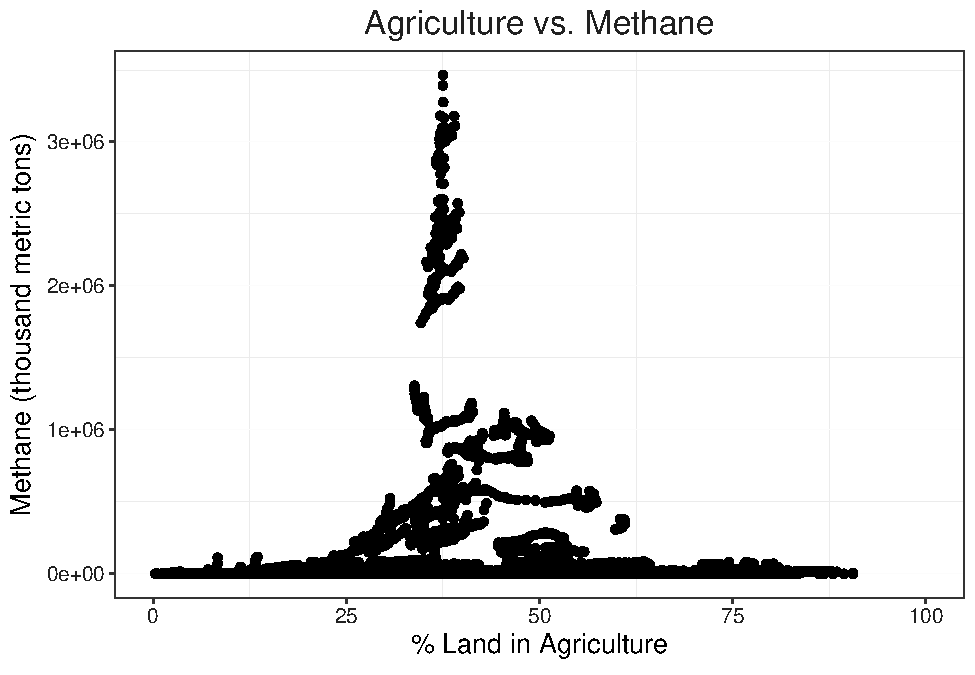
\includegraphics{Marx_ENV872_Project_files/figure-latex/unnamed-chunk-4-1.pdf}

\begin{verbatim}
## Warning: Removed 10791 rows containing missing values (geom_point).
\end{verbatim}

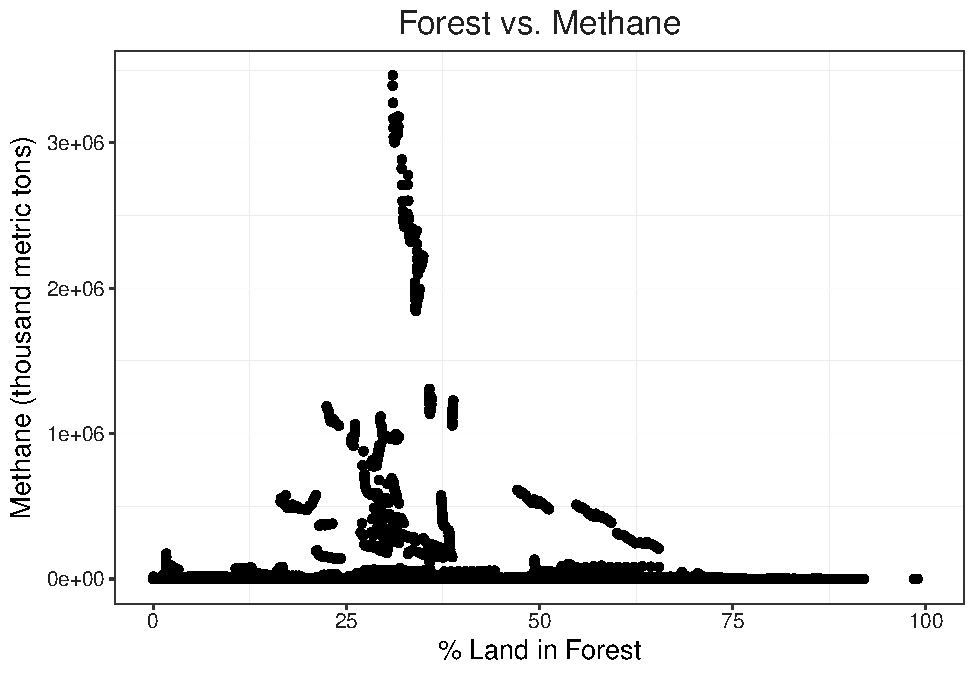
\includegraphics{Marx_ENV872_Project_files/figure-latex/unnamed-chunk-4-2.pdf}

\begin{verbatim}
## Warning: Removed 10791 rows containing missing values (geom_point).

## Warning: Removed 6297 rows containing missing values (geom_point).
\end{verbatim}

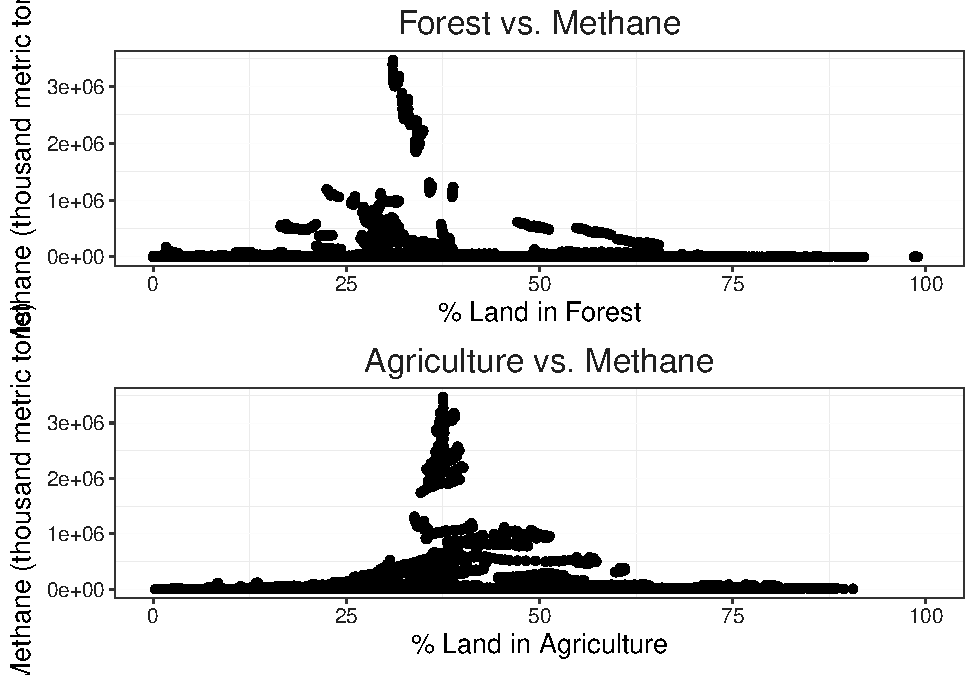
\includegraphics{Marx_ENV872_Project_files/figure-latex/unnamed-chunk-4-3.pdf}

```

\begin{Shaded}
\begin{Highlighting}[]
\NormalTok{AgVCarbon <-}\StringTok{ }
\StringTok{  }\KeywordTok{ggplot}\NormalTok{(WorldBank_Spread) }\OperatorTok{+}\StringTok{ }
\StringTok{  }\KeywordTok{geom_point}\NormalTok{(}\KeywordTok{aes}\NormalTok{(}\DataTypeTok{x =}\NormalTok{ Agriculture, }\DataTypeTok{y =}\NormalTok{ CO2Emissions)) }\OperatorTok{+}
\StringTok{  }\KeywordTok{ggtitle}\NormalTok{(}\StringTok{"Agriculture vs. Carbon"}\NormalTok{) }\OperatorTok{+}
\StringTok{  }\KeywordTok{ylab}\NormalTok{(}\KeywordTok{expression}\NormalTok{(}\StringTok{"Carbon"}\NormalTok{)) }\OperatorTok{+}
\StringTok{  }\KeywordTok{xlab}\NormalTok{(}\KeywordTok{expression}\NormalTok{(}\StringTok{"% Land in Agriculture"}\NormalTok{)) }\OperatorTok{+}
\StringTok{  }\KeywordTok{scale_x_continuous}\NormalTok{(}\DataTypeTok{limits =} \KeywordTok{c}\NormalTok{(}\DecValTok{0}\NormalTok{,}\DecValTok{100}\NormalTok{)) }\OperatorTok{+}
\StringTok{  }\KeywordTok{scale_color_manual}\NormalTok{(}\DataTypeTok{values =} \KeywordTok{c}\NormalTok{(}\StringTok{"brown"}\NormalTok{, }\StringTok{"goldenrod"}\NormalTok{)) }
\KeywordTok{print}\NormalTok{(AgVCarbon)}
\end{Highlighting}
\end{Shaded}

\begin{verbatim}
## Warning: Removed 3900 rows containing missing values (geom_point).
\end{verbatim}

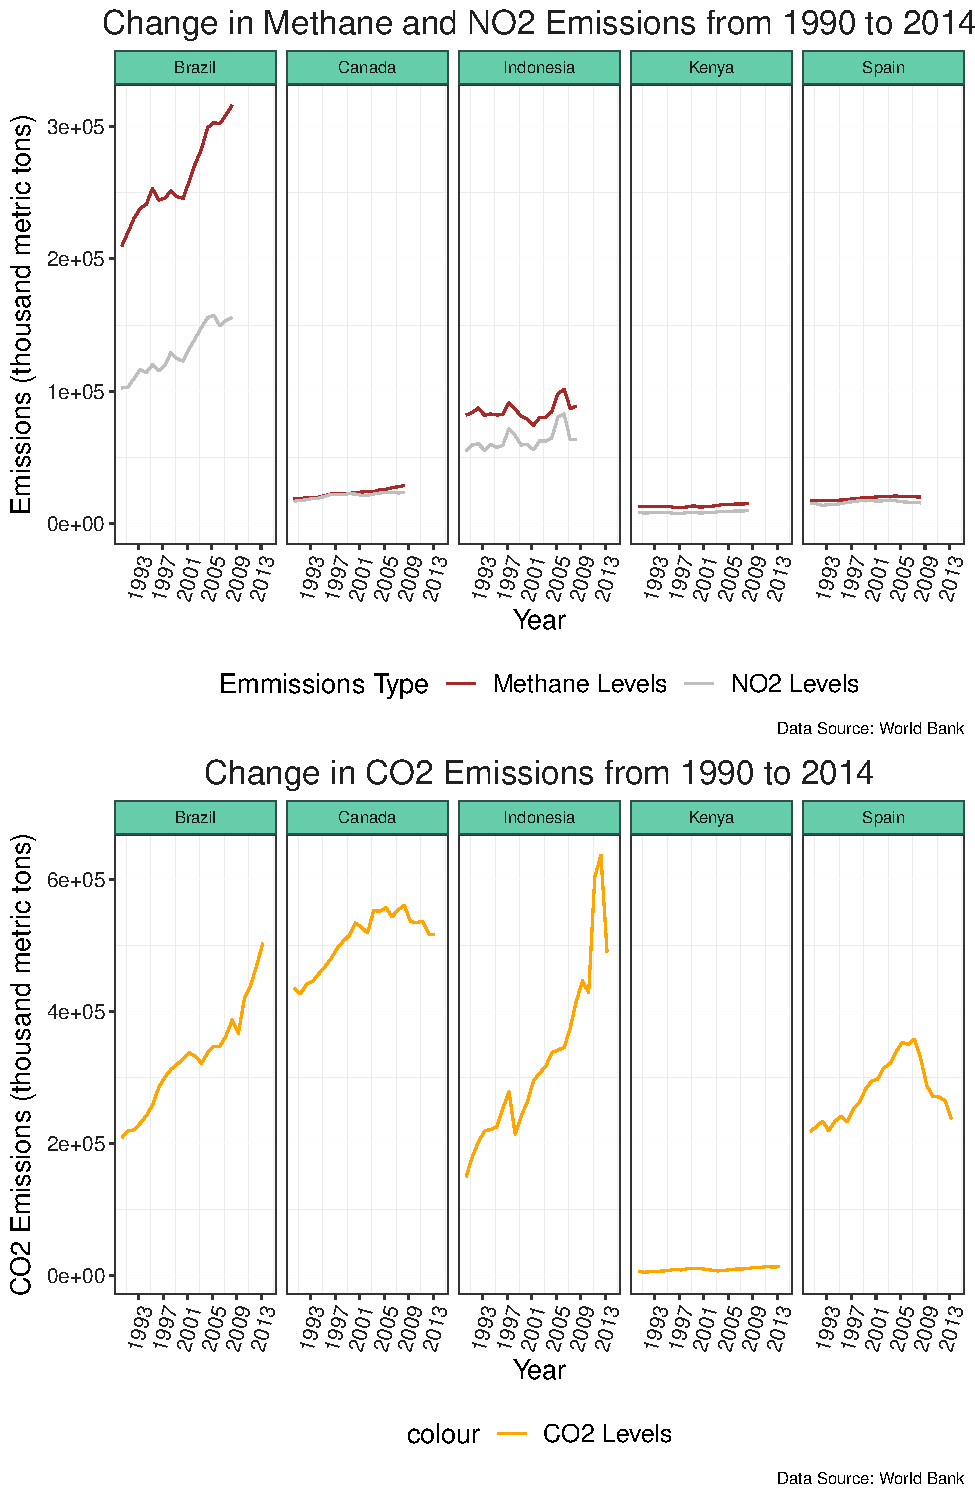
\includegraphics{Marx_ENV872_Project_files/figure-latex/unnamed-chunk-5-1.pdf}

\begin{Shaded}
\begin{Highlighting}[]
\NormalTok{ForestVCarbon <-}\StringTok{ }
\StringTok{  }\KeywordTok{ggplot}\NormalTok{(WorldBank_Spread) }\OperatorTok{+}\StringTok{ }
\StringTok{  }\KeywordTok{geom_point}\NormalTok{(}\KeywordTok{aes}\NormalTok{(}\DataTypeTok{x =}\NormalTok{ Forest, }\DataTypeTok{y =}\NormalTok{ CO2Emissions)) }\OperatorTok{+}
\StringTok{  }\KeywordTok{ggtitle}\NormalTok{(}\StringTok{"Forest vs. Carbon"}\NormalTok{) }\OperatorTok{+}
\StringTok{  }\KeywordTok{ylab}\NormalTok{(}\KeywordTok{expression}\NormalTok{(}\StringTok{"Carbon"}\NormalTok{)) }\OperatorTok{+}
\StringTok{  }\KeywordTok{xlab}\NormalTok{(}\KeywordTok{expression}\NormalTok{(}\StringTok{"% Land in Forest"}\NormalTok{)) }\OperatorTok{+}
\StringTok{  }\KeywordTok{scale_x_continuous}\NormalTok{(}\DataTypeTok{limits =} \KeywordTok{c}\NormalTok{(}\DecValTok{0}\NormalTok{,}\DecValTok{100}\NormalTok{)) }
\KeywordTok{print}\NormalTok{(ForestVCarbon)}
\end{Highlighting}
\end{Shaded}

\begin{verbatim}
## Warning: Removed 9616 rows containing missing values (geom_point).
\end{verbatim}

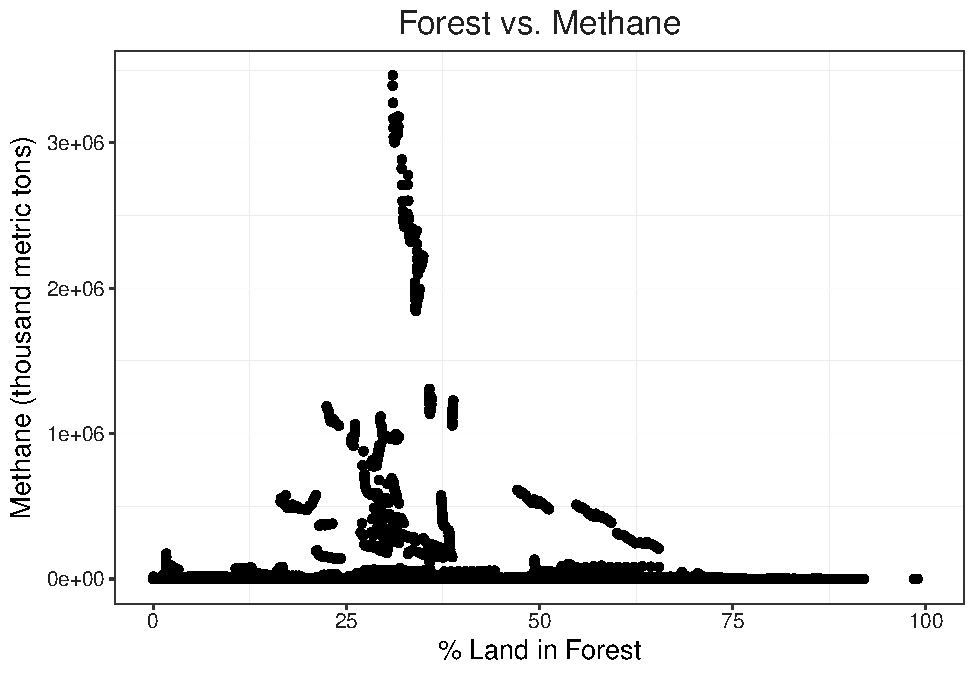
\includegraphics{Marx_ENV872_Project_files/figure-latex/unnamed-chunk-5-2.pdf}

\begin{verbatim}
## Warning: Removed 35 rows containing missing values (geom_path).

## Warning: Removed 35 rows containing missing values (geom_path).
\end{verbatim}

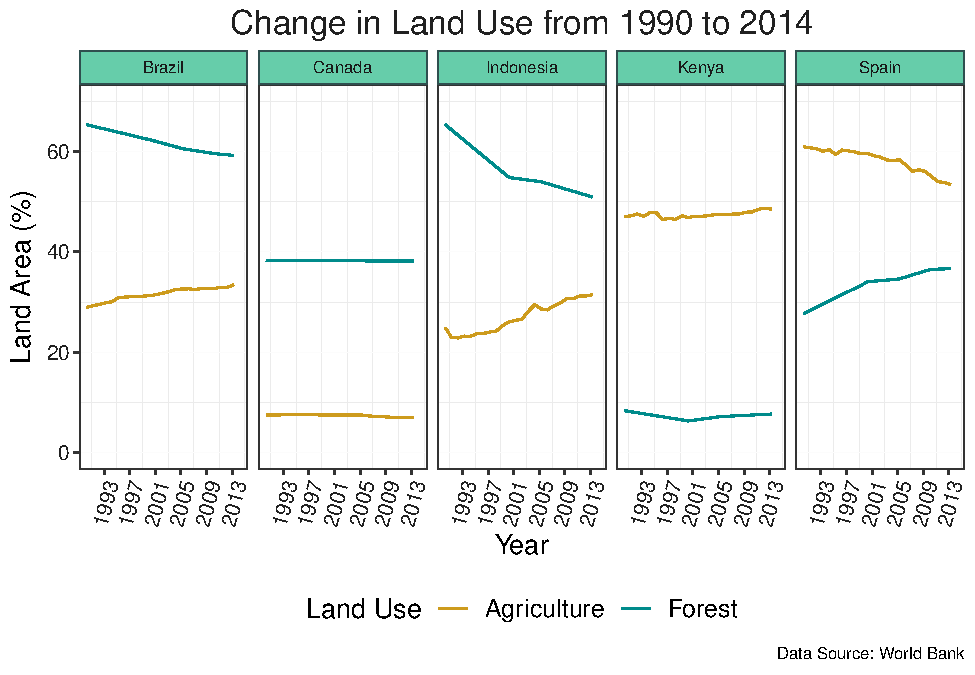
\includegraphics{Marx_ENV872_Project_files/figure-latex/unnamed-chunk-6-1.pdf}

\begin{verbatim}
## Warning: Removed 40 rows containing missing values (geom_path).

## Warning: Removed 40 rows containing missing values (geom_path).
\end{verbatim}

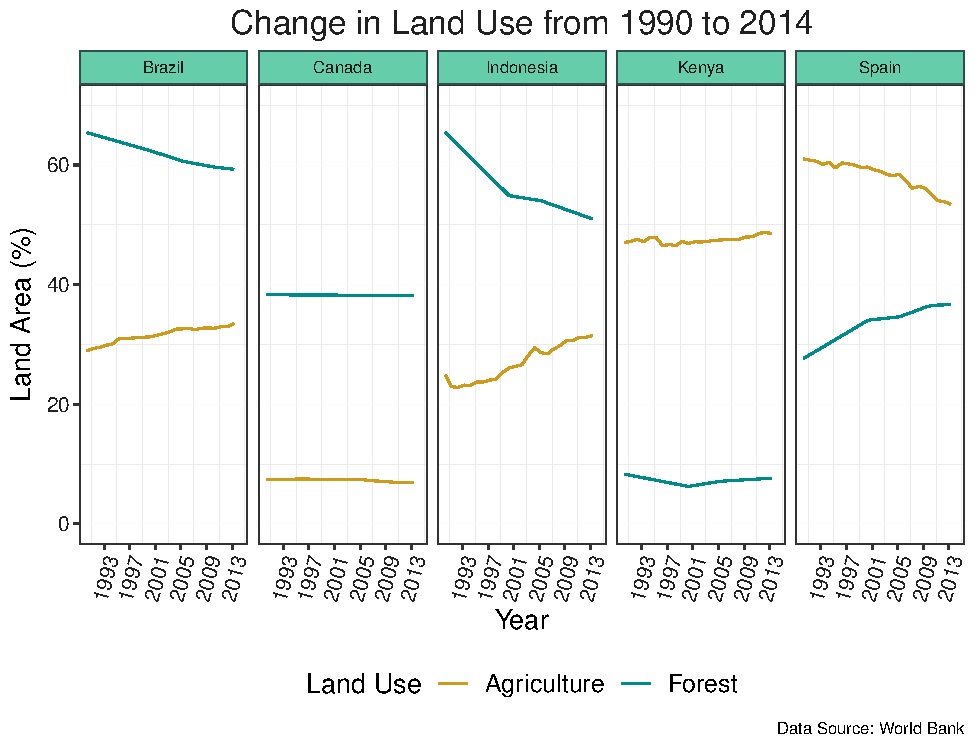
\includegraphics{Marx_ENV872_Project_files/figure-latex/unnamed-chunk-7-1.pdf}

\begin{verbatim}

\end{verbatim}

\subsection{Warning: Removed 35 rows containing missing values
(geom\_path).}\label{warning-removed-35-rows-containing-missing-values-geom_path.}

\begin{verbatim}

![](Marx_ENV872_Project_files/figure-latex/unnamed-chunk-8-1.pdf)<!-- --> 

\end{verbatim}

\subsection{Warning: Removed 35 rows containing missing values
(geom\_path).}\label{warning-removed-35-rows-containing-missing-values-geom_path.-1}

\subsection{Warning: Removed 35 rows containing missing values
(geom\_path).}\label{warning-removed-35-rows-containing-missing-values-geom_path.-2}

```

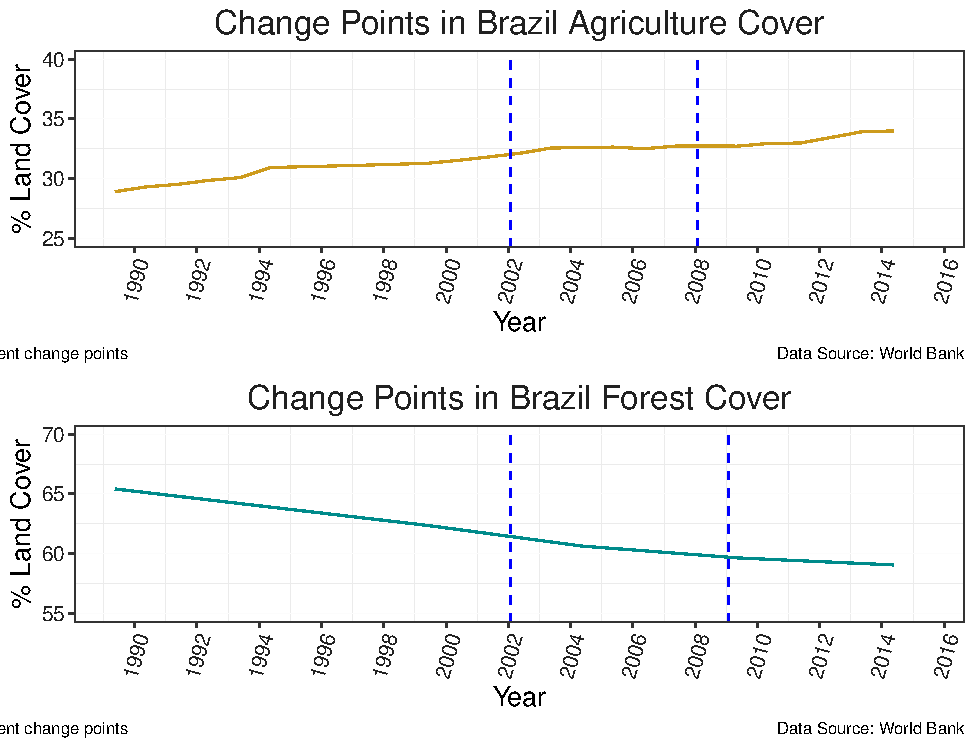
\includegraphics{Marx_ENV872_Project_files/figure-latex/unnamed-chunk-9-1.pdf}

\newpage

\section{Analysis}\label{analysis}

\begin{Shaded}
\begin{Highlighting}[]
\CommentTok{#Statistical Test 1: How has forest changed over time }
\NormalTok{Forest.Time1 <-}\StringTok{ }\KeywordTok{gls}\NormalTok{(}\DataTypeTok{data =}\NormalTok{ WB_Spread, }
\NormalTok{                    Forest }\OperatorTok{~}\StringTok{ }\NormalTok{Year,}
                    \DataTypeTok{method =} \StringTok{"REML"}\NormalTok{)}
\KeywordTok{summary}\NormalTok{(Forest.Time1)}
\end{Highlighting}
\end{Shaded}

\begin{verbatim}
## Generalized least squares fit by REML
##   Model: Forest ~ Year 
##   Data: WB_Spread 
##        AIC      BIC    logLik
##   49977.96 49997.13 -24985.98
## 
## Coefficients:
##                Value Std.Error   t-value p-value
## (Intercept) 83.48146  5.839645 14.295639       0
## Year        -0.00425  0.000533 -7.987907       0
## 
##  Correlation: 
##      (Intr)
## Year -0.984
## 
## Standardized residuals:
##         Min          Q1         Med          Q3         Max 
## -0.74247841 -0.33743857 -0.09641382  0.15552883 16.46833243 
## 
## Residual standard error: 69.98862 
## Degrees of freedom: 4408 total; 4406 residual
\end{verbatim}

\begin{Shaded}
\begin{Highlighting}[]
\NormalTok{Forest.Time2 <-}\StringTok{ }\KeywordTok{lme}\NormalTok{(}\DataTypeTok{data =}\NormalTok{ WB_Spread,}
\NormalTok{                Forest }\OperatorTok{~}\StringTok{ }\NormalTok{Year,}
                \DataTypeTok{random =} \OperatorTok{~}\DecValTok{1}\OperatorTok{|}\StringTok{ }\NormalTok{Country)}
\KeywordTok{summary}\NormalTok{(Forest.Time2)}
\end{Highlighting}
\end{Shaded}

\begin{verbatim}
## Linear mixed-effects model fit by REML
##  Data: WB_Spread 
##        AIC      BIC    logLik
##   49431.95 49457.52 -24711.98
## 
## Random effects:
##  Formula: ~1 | Country
##         (Intercept) Residual
## StdDev:    30.52692 62.84915
## 
## Fixed effects: Forest ~ Year 
##                Value Std.Error   DF   t-value p-value
## (Intercept) 82.96649  5.653843 4163 14.674352       0
## Year        -0.00421  0.000482 4163 -8.743567       0
##  Correlation: 
##      (Intr)
## Year -0.923
## 
## Standardized Within-Group Residuals:
##         Min          Q1         Med          Q3         Max 
## -2.55113019 -0.14187377 -0.01873545  0.09332491 16.07509035 
## 
## Number of Observations: 4408
## Number of Groups: 244
\end{verbatim}

A fixed effects model was used to see how land percetnage of forest area
accross the whoel data set changes over time. The results show that, on
average, forest decreases by -.00485\% each year. Was not worride about
seasonality of the data because there is only one data point per year.
As such, I did not calculate autocorrelations. I did add country as a
random effect.

\begin{Shaded}
\begin{Highlighting}[]
\NormalTok{For.Ag.}\DecValTok{1}\NormalTok{ <-}\StringTok{ }\KeywordTok{gls}\NormalTok{(}\DataTypeTok{data =}\NormalTok{ WB_Spread, }
\NormalTok{                    Forest }\OperatorTok{~}\StringTok{ }\NormalTok{Year }\OperatorTok{+}\StringTok{ }\NormalTok{Agriculture,}
                    \DataTypeTok{method =} \StringTok{"REML"}\NormalTok{)}
\KeywordTok{summary}\NormalTok{(For.Ag.}\DecValTok{1}\NormalTok{)}
\end{Highlighting}
\end{Shaded}

\begin{verbatim}
## Generalized least squares fit by REML
##   Model: Forest ~ Year + Agriculture 
##   Data: WB_Spread 
##        AIC      BIC    logLik
##   49908.57 49934.13 -24950.29
## 
## Coefficients:
##                 Value Std.Error   t-value p-value
## (Intercept) 100.30274  6.103018 16.434939       0
## Year         -0.00423  0.000528 -8.007157       0
## Agriculture  -0.44673  0.051202 -8.724865       0
## 
##  Correlation: 
##             (Intr) Year  
## Year        -0.931       
## Agriculture -0.316 -0.006
## 
## Standardized residuals:
##         Min          Q1         Med          Q3         Max 
## -0.98942500 -0.26448939 -0.05947803  0.14053065 16.59420967 
## 
## Residual standard error: 69.39948 
## Degrees of freedom: 4408 total; 4405 residual
\end{verbatim}

\begin{Shaded}
\begin{Highlighting}[]
\NormalTok{For.Ag.}\DecValTok{2}\NormalTok{ <-}\StringTok{  }\KeywordTok{lme}\NormalTok{(}\DataTypeTok{data =}\NormalTok{ WB_Spread,}
\NormalTok{              Forest }\OperatorTok{~}\StringTok{ }\NormalTok{Year }\OperatorTok{+}\StringTok{ }\NormalTok{Agriculture,}
              \DataTypeTok{random =} \OperatorTok{~}\DecValTok{1}\OperatorTok{|}\StringTok{ }\NormalTok{Country)}
\KeywordTok{summary}\NormalTok{(For.Ag.}\DecValTok{2}\NormalTok{)}
\end{Highlighting}
\end{Shaded}

\begin{verbatim}
## Linear mixed-effects model fit by REML
##  Data: WB_Spread 
##       AIC      BIC    logLik
##   49413.7 49445.65 -24701.85
## 
## Random effects:
##  Formula: ~1 | Country
##         (Intercept) Residual
## StdDev:    29.32764 62.80075
## 
## Fixed effects: Forest ~ Year + Agriculture 
##                 Value Std.Error   DF   t-value p-value
## (Intercept) 101.78896  6.830290 4162 14.902583       0
## Year         -0.00421  0.000481 4162 -8.754338       0
## Agriculture  -0.49055  0.101138 4162 -4.850333       0
##  Correlation: 
##             (Intr) Year  
## Year        -0.763       
## Agriculture -0.568  0.000
## 
## Standardized Within-Group Residuals:
##         Min          Q1         Med          Q3         Max 
## -2.53066671 -0.13903414 -0.01968184  0.09295492 16.10850732 
## 
## Number of Observations: 4408
## Number of Groups: 244
\end{verbatim}

\begin{Shaded}
\begin{Highlighting}[]
\CommentTok{#anova(Forest.Fixed, Test2) # Said: fitted objects with different fixed effects. REML comparisons are not meaningful.}
\end{Highlighting}
\end{Shaded}

Results of first set of tests:

I am interested in whether access to electricity or the levels of
renewable energy produced in countries have a relationship with
deforestation. This is becasue a lack of electricity could drive the use
of forest biomass products as an energy source. Electricity access
appears to have a negative impact on forest (-.333) which may be because
electricity is needed for some agricultural operations, or electricity
is being produced via biofuels, the production of which might require
more forest to be converted to agricultural land. ( \ref{fig:fig3})

With that theory in mind, I was interested in whether there might be a
relationship between forested land and renewable energy because energy
produced from biomass is considered to be renewable. However, the result
of my gls revealed that a 1 unit increase in renewable energy is
associated with a .18\% increase in forest land, meaning the production
of biofule is likely not a main driver of deforestation.

\begin{Shaded}
\begin{Highlighting}[]
\CommentTok{#Looking at Electricity Accesss and Renewable Energy as a Drive of the Ag. / Forest Tradeoff}

\CommentTok{#Add Electricity }
\NormalTok{Forest.Ag.Elec <-}\StringTok{ }\KeywordTok{gls}\NormalTok{(}\DataTypeTok{data =}\NormalTok{ WB_Spread, }
\NormalTok{                    Forest }\OperatorTok{~}\StringTok{ }\NormalTok{Year }\OperatorTok{+}\StringTok{ }\NormalTok{Agriculture }\OperatorTok{+}\StringTok{ }\NormalTok{ElectricityAccess,}
                    \DataTypeTok{method =} \StringTok{"REML"}\NormalTok{)}
\NormalTok{Forest.Ag.Elec}
\end{Highlighting}
\end{Shaded}

\begin{verbatim}
## Generalized least squares fit by REML
##   Model: Forest ~ Year + Agriculture + ElectricityAccess 
##   Data: WB_Spread 
##   Log-restricted-likelihood: -24906.59
## 
## Coefficients:
##       (Intercept)              Year       Agriculture ElectricityAccess 
##     117.273716122      -0.003583843      -0.514782445      -0.299412308 
## 
## Degrees of freedom: 4408 total; 4404 residual
## Residual standard error: 68.68236
\end{verbatim}

\begin{Shaded}
\begin{Highlighting}[]
\CommentTok{#Electricity only }
\NormalTok{Forest.Elec <-}\StringTok{ }\KeywordTok{gls}\NormalTok{(}\DataTypeTok{data =}\NormalTok{ WB_Spread, }
\NormalTok{                    Forest }\OperatorTok{~}\StringTok{ }\NormalTok{Year }\OperatorTok{+}\StringTok{ }\NormalTok{ElectricityAccess,}
                    \DataTypeTok{method =} \StringTok{"REML"}\NormalTok{)}
\NormalTok{Forest.Elec}
\end{Highlighting}
\end{Shaded}

\begin{verbatim}
## Generalized least squares fit by REML
##   Model: Forest ~ Year + ElectricityAccess 
##   Data: WB_Spread 
##   Log-restricted-likelihood: -24954.6
## 
## Coefficients:
##       (Intercept)              Year ElectricityAccess 
##      95.826798295      -0.003705033      -0.256536944 
## 
## Degrees of freedom: 4408 total; 4405 residual
## Residual standard error: 69.4595
\end{verbatim}

\begin{Shaded}
\begin{Highlighting}[]
\NormalTok{Forest.RE <-}\StringTok{ }\KeywordTok{gls}\NormalTok{(}\DataTypeTok{data =}\NormalTok{ WB_Spread, }
\NormalTok{                    Forest }\OperatorTok{~}\StringTok{ }\NormalTok{Year }\OperatorTok{+}\StringTok{ }\NormalTok{RenewableElectricity,}
                    \DataTypeTok{method =} \StringTok{"REML"}\NormalTok{)}
\NormalTok{Forest.RE}
\end{Highlighting}
\end{Shaded}

\begin{verbatim}
## Generalized least squares fit by REML
##   Model: Forest ~ Year + RenewableElectricity 
##   Data: WB_Spread 
##   Log-restricted-likelihood: -24969.59
## 
## Coefficients:
##          (Intercept)                 Year RenewableElectricity 
##         75.893689686         -0.004120715          0.199889723 
## 
## Degrees of freedom: 4408 total; 4405 residual
## Residual standard error: 69.69694
\end{verbatim}

\begin{Shaded}
\begin{Highlighting}[]
\CommentTok{#On that note, }

\CommentTok{# Regression w/o time }
\NormalTok{Reg1 <-}\StringTok{ }\KeywordTok{lm}\NormalTok{(Forest }\OperatorTok{~}\StringTok{ }\NormalTok{Agriculture, WorldBank_Spread)}
\NormalTok{Reg1}
\end{Highlighting}
\end{Shaded}

\begin{verbatim}
## 
## Call:
## lm(formula = Forest ~ Agriculture, data = WorldBank_Spread)
## 
## Coefficients:
## (Intercept)  Agriculture  
##     52.5762      -0.4444
\end{verbatim}

\begin{Shaded}
\begin{Highlighting}[]
\CommentTok{#A 1 unit increas in agriculture leads to a -.44 decrease in forest }
\end{Highlighting}
\end{Shaded}

As a second statistical test I used Pettit's test, a nonparametric test
that determines if there is a shift in the central tendency of the time
series. It also determines at what point in time the changepoint occurs.
I used this to see if there was a point in time in particular where
these seemed to be a noticeable change in forest cover. I applied the
test to Brazil which graphically appears to have change points to see if
1) there was a change poing for agriculture and forest and 2) to see if
the change points occured in the same year for each.

\begin{Shaded}
\begin{Highlighting}[]
\CommentTok{#Statistical Test 2: Pettitts Test: Looking at Change Points in the Data}

\CommentTok{#Statistical Test 2: Any change points for full forest data?}
\KeywordTok{pettitt.test}\NormalTok{(WB_Spread}\OperatorTok{$}\NormalTok{Forest)}
\end{Highlighting}
\end{Shaded}

\begin{verbatim}
## 
##  Pettitt's test for single change-point detection
## 
## data:  WB_Spread$Forest
## U* = 463360, p-value = 5.895e-07
## alternative hypothesis: two.sided
## sample estimates:
## probable change point at time K 
##                            1739
\end{verbatim}

\begin{Shaded}
\begin{Highlighting}[]
\CommentTok{#Probable change point at time 1428 which doesn't exist.}


\CommentTok{#Changes in Brazil Forest}
\KeywordTok{pettitt.test}\NormalTok{(WB_Brazil}\OperatorTok{$}\NormalTok{Forest)}
\end{Highlighting}
\end{Shaded}

\begin{verbatim}
## 
##  Pettitt's test for single change-point detection
## 
## data:  WB_Brazil$Forest
## U* = 90, p-value = 0.002386
## alternative hypothesis: two.sided
## sample estimates:
## probable change point at time K                            <NA> 
##                               9                              10
\end{verbatim}

\begin{Shaded}
\begin{Highlighting}[]
\CommentTok{#9 (of 19): 1998; p-value .048 (significant at the .05 level)}

\KeywordTok{pettitt.test}\NormalTok{(WB_Brazil}\OperatorTok{$}\NormalTok{Forest[}\DecValTok{9}\OperatorTok{:}\DecValTok{19}\NormalTok{])}
\end{Highlighting}
\end{Shaded}

\begin{verbatim}
## 
##  Pettitt's test for single change-point detection
## 
## data:  WB_Brazil$Forest[9:19]
## U* = 30, p-value = 0.04852
## alternative hypothesis: two.sided
## sample estimates:
## probable change point at time K                            <NA> 
##                               5                               6
\end{verbatim}

\begin{Shaded}
\begin{Highlighting}[]
\CommentTok{#Changes in Brazil Agriculture }
\CommentTok{#5 (9+5 = 14: 2003); p-value .0023852 (significant at the .01 level)}

\KeywordTok{pettitt.test}\NormalTok{(WB_Brazil}\OperatorTok{$}\NormalTok{Forest[}\DecValTok{14}\OperatorTok{:}\DecValTok{19}\NormalTok{])}
\end{Highlighting}
\end{Shaded}

\begin{verbatim}
## 
##  Pettitt's test for single change-point detection
## 
## data:  WB_Brazil$Forest[14:19]
## U* = 9, p-value = 0.2907
## alternative hypothesis: two.sided
## sample estimates:
## probable change point at time K 
##                               3
\end{verbatim}

\begin{Shaded}
\begin{Highlighting}[]
\CommentTok{#3 14 + 3 = 17: 2006 (p-value .29: not significant)}

\KeywordTok{pettitt.test}\NormalTok{(WB_Brazil}\OperatorTok{$}\NormalTok{Agriculture)}
\end{Highlighting}
\end{Shaded}

\begin{verbatim}
## 
##  Pettitt's test for single change-point detection
## 
## data:  WB_Brazil$Agriculture
## U* = 90, p-value = 0.002386
## alternative hypothesis: two.sided
## sample estimates:
## probable change point at time K                            <NA> 
##                               9                              10
\end{verbatim}

\begin{Shaded}
\begin{Highlighting}[]
\CommentTok{#9 (of 19): 1998; p-value .002386 (significant at the .01 level)}

\KeywordTok{pettitt.test}\NormalTok{(WB_Brazil}\OperatorTok{$}\NormalTok{Agriculture[}\DecValTok{9}\OperatorTok{:}\DecValTok{19}\NormalTok{])}
\end{Highlighting}
\end{Shaded}

\begin{verbatim}
## 
##  Pettitt's test for single change-point detection
## 
## data:  WB_Brazil$Agriculture[9:19]
## U* = 30, p-value = 0.04852
## alternative hypothesis: two.sided
## sample estimates:
## probable change point at time K                            <NA> 
##                               5                               6
\end{verbatim}

\begin{Shaded}
\begin{Highlighting}[]
\CommentTok{#5 (9+5 = 14: 2003); p-value .04852 (significant at the .05 level}

\KeywordTok{pettitt.test}\NormalTok{(WB_Brazil}\OperatorTok{$}\NormalTok{Agriculture[}\DecValTok{14}\OperatorTok{:}\DecValTok{19}\NormalTok{])}
\end{Highlighting}
\end{Shaded}

\begin{verbatim}
## 
##  Pettitt's test for single change-point detection
## 
## data:  WB_Brazil$Agriculture[14:19]
## U* = 6, p-value = 0.8487
## alternative hypothesis: two.sided
## sample estimates:
## probable change point at time K 
##                               2
\end{verbatim}

\begin{Shaded}
\begin{Highlighting}[]
\CommentTok{#2 (14 +2 = 16) p-value .8487 (not significant)}
\end{Highlighting}
\end{Shaded}

Pettitt's applied to a single country (Brazil) initially detects a
change point in Forest and Agriculture in the same year. The change for
both was in place 9, which is the year 1998. The significant change
points for agriculture and forest in Brazil occured in the same years
(1998 and 2003), furhter supporting the notion that there is a
relationship between the two.

{[}Make a graph of Brazil that shows the change points{]}

The next series of tests address the question: Is there a relationship
between land uses (agriculture or forest) and levels of CO2, methane,
and NO3 emissions?

\begin{Shaded}
\begin{Highlighting}[]
\CommentTok{#Statistical Test 3.1: Agriculture & Methane Emmissions}

\NormalTok{AgMethane <-}\StringTok{ }\KeywordTok{gls}\NormalTok{(}\DataTypeTok{data =}\NormalTok{ WB_Spread,}
\NormalTok{                 Ag.Methane }\OperatorTok{~}\StringTok{ }\NormalTok{Year }\OperatorTok{+}\StringTok{ }\NormalTok{Agriculture,}
                 \DataTypeTok{method =} \StringTok{"REML"}\NormalTok{)}
\NormalTok{AgMethane}
\end{Highlighting}
\end{Shaded}

\begin{verbatim}
## Generalized least squares fit by REML
##   Model: Ag.Methane ~ Year + Agriculture 
##   Data: WB_Spread 
##   Log-restricted-likelihood: -63169.07
## 
## Coefficients:
##  (Intercept)         Year  Agriculture 
## 1.172434e+05 3.206730e-02 5.445887e+02 
## 
## Degrees of freedom: 4408 total; 4405 residual
## Residual standard error: 406812.4
\end{verbatim}

\begin{Shaded}
\begin{Highlighting}[]
\CommentTok{#Statistica Test 3.2: Forest & Methane Emmissions}
\NormalTok{ForestMethane <-}\StringTok{ }\KeywordTok{gls}\NormalTok{(}\DataTypeTok{data =}\NormalTok{ WB_Spread, }
\NormalTok{                  Ag.Methane }\OperatorTok{~}\StringTok{ }\NormalTok{Year }\OperatorTok{+}\StringTok{ }\NormalTok{Forest,}
                  \DataTypeTok{method =} \StringTok{"REML"}\NormalTok{)}
\KeywordTok{summary}\NormalTok{(ForestMethane)}
\end{Highlighting}
\end{Shaded}

\begin{verbatim}
## Generalized least squares fit by REML
##   Model: Ag.Methane ~ Year + Forest 
##   Data: WB_Spread 
##        AIC      BIC    logLik
##   126331.7 126357.3 -63161.87
## 
## Coefficients:
##                 Value Std.Error  t-value p-value
## (Intercept) 104949.59  34655.09 3.028404  0.0025
## Year             1.73      3.11 0.557427  0.5773
## Forest         392.90     87.40 4.495392  0.0000
## 
##  Correlation: 
##        (Intr) Year  
## Year   -0.980       
## Forest -0.211  0.119
## 
## Standardized residuals:
##        Min         Q1        Med         Q3        Max 
## -0.9349863 -0.3368465 -0.3079788 -0.2493750  8.1856088 
## 
## Residual standard error: 406034.1 
## Degrees of freedom: 4408 total; 4405 residual
\end{verbatim}

\begin{Shaded}
\begin{Highlighting}[]
\CommentTok{#Statistical Test 3.3: Interaction of Forest and Agriculture on Methane Emissions #These are probably correleated. Run a VIF Test. }
\NormalTok{Int.Methane <-}\StringTok{  }\KeywordTok{gls}\NormalTok{(}\DataTypeTok{data =}\NormalTok{ WB_Spread,}
\NormalTok{                    Ag.Methane }\OperatorTok{~}\StringTok{ }\NormalTok{Year }\OperatorTok{+}\StringTok{ }\NormalTok{Forest }\OperatorTok{*}\StringTok{ }\NormalTok{Agriculture,}
                    \DataTypeTok{method =} \StringTok{"REML"}\NormalTok{)}
\NormalTok{Int.Methane }
\end{Highlighting}
\end{Shaded}

\begin{verbatim}
## Generalized least squares fit by REML
##   Model: Ag.Methane ~ Year + Forest * Agriculture 
##   Data: WB_Spread 
##   Log-restricted-likelihood: -63123.24
## 
## Coefficients:
##        (Intercept)               Year             Forest 
##      170978.276563           2.186635       -2547.247815 
##        Agriculture Forest:Agriculture 
##       -1627.888779          81.435201 
## 
## Degrees of freedom: 4408 total; 4403 residual
## Residual standard error: 403492.6
\end{verbatim}

As the percetage of land under agriculture increases by 1, methane
emissions increase by 6.57 thousand metric tons.

As Forest land increases by 1\%, methane emissions increase by .035
thoushand metric tons (or 35 metirc tons), meaning that deforestation is
not strongly related to methan emissions.

However, if the interaction of forest and agriculture land cover is
considered, an increase of 1 leads to an increase of 98.86 thousand
metric tons of methane.

\begin{Shaded}
\begin{Highlighting}[]
\CommentTok{#Carbon Emissions Tests }

\CommentTok{#Test 4.1: Forest and Carbon}
\NormalTok{Forest.CO2 <-}\StringTok{ }\KeywordTok{gls}\NormalTok{(}\DataTypeTok{data =}\NormalTok{ WB_Spread, }
\NormalTok{                  CO2Emissions }\OperatorTok{~}\StringTok{ }\NormalTok{Year }\OperatorTok{+}\StringTok{ }\NormalTok{Forest,}
                  \DataTypeTok{method =} \StringTok{"REML"}\NormalTok{)}
\NormalTok{Forest.CO2 }
\end{Highlighting}
\end{Shaded}

\begin{verbatim}
## Generalized least squares fit by REML
##   Model: CO2Emissions ~ Year + Forest 
##   Data: WB_Spread 
##   Log-restricted-likelihood: -71822.3
## 
## Coefficients:
##  (Intercept)         Year       Forest 
## 311972.83203     54.86307     30.35953 
## 
## Degrees of freedom: 4408 total; 4405 residual
## Residual standard error: 2900052
\end{verbatim}

\begin{Shaded}
\begin{Highlighting}[]
\CommentTok{#Test 4.2: Agriculture and Carbon }
\NormalTok{Ag.CO2 <-}\StringTok{ }\KeywordTok{gls}\NormalTok{(}\DataTypeTok{data =}\NormalTok{ WB_Spread,}
\NormalTok{                 CO2Emissions }\OperatorTok{~}\StringTok{ }\NormalTok{Year }\OperatorTok{+}\StringTok{ }\NormalTok{Agriculture,}
                 \DataTypeTok{method =} \StringTok{"REML"}\NormalTok{)}
\NormalTok{Ag.CO2 }
\end{Highlighting}
\end{Shaded}

\begin{verbatim}
## Generalized least squares fit by REML
##   Model: CO2Emissions ~ Year + Agriculture 
##   Data: WB_Spread 
##   Log-restricted-likelihood: -71820.95
## 
## Coefficients:
##  (Intercept)         Year  Agriculture 
## 274157.42618     54.67258   1071.59529 
## 
## Degrees of freedom: 4408 total; 4405 residual
## Residual standard error: 2899970
\end{verbatim}

\begin{Shaded}
\begin{Highlighting}[]
\CommentTok{#Test 4.3: Interaction of Forest & Agriculture on Carbon }
\NormalTok{Int.CO2 <-}\StringTok{ }\KeywordTok{gls}\NormalTok{(}\DataTypeTok{data =}\NormalTok{ WB_Spread,}
\NormalTok{                    CO2Emissions }\OperatorTok{~}\StringTok{ }\NormalTok{Year }\OperatorTok{+}\StringTok{ }\NormalTok{Forest }\OperatorTok{*}\StringTok{ }\NormalTok{Agriculture,}
                    \DataTypeTok{method =} \StringTok{"REML"}\NormalTok{)}
\NormalTok{Int.CO2 }
\end{Highlighting}
\end{Shaded}

\begin{verbatim}
## Generalized least squares fit by REML
##   Model: CO2Emissions ~ Year + Forest * Agriculture 
##   Data: WB_Spread 
##   Log-restricted-likelihood: -71789.87
## 
## Coefficients:
##        (Intercept)               Year             Forest 
##       847291.77408           57.25021       -17883.04480 
##        Agriculture Forest:Agriculture 
##       -13175.94334          492.65459 
## 
## Degrees of freedom: 4408 total; 4403 residual
## Residual standard error: 2888536
\end{verbatim}

1\% increase in forest leads to a -235.25 decrease in CO2. 1\% increase
in Ag. leads to an increase of 1493 kt of carbon. Interaction: How do
you interpret?

\newpage

\section{Summary and Conclusions}\label{summary-and-conclusions}


\end{document}
